\chapter{Introduction to GLSL}

\section{Shaders in OpenGL}

We've seen in the previous section how geometry can be specified and how a draw call can be issued in OpenGL. Now we address two other important issues in rendering images: where does the object appear in the scene, and what colour(s) does it have? Oh, and how do we ensure an image comes out of the pipeline in the first place?

All of these are accomplished through something known as a \emph{Shader}. In OpenGL, a Shader is a small program that runs on the GPU. Usually shaders are run once in their entirety for every single input item they process. In the case of a vertex shader, this would be vertices. There exist a number of types of Shaders for different purposes. 

Shaders are commonly invoked many times (in the order of millions) to render even a single frame. There's a range of different kinds of Shaders, but most of them are irrelevant unless you're trying to do something very advanced.

In practice, you'll commonly only be using two particular types of Shaders:

\begin{itemize}
  \item The Vertex Shader
  \item The Fragment Shader
\end{itemize}

As we've seen before, these shaders form an integral part of the rendering pipeline, and we're required to specify them before issuing any draw calls. For reference, here's the diagram showing the pipeline we've seen in chapter 1. Note where the Vertex and Fragment shaders are located in the pipeline.

\centerline {
	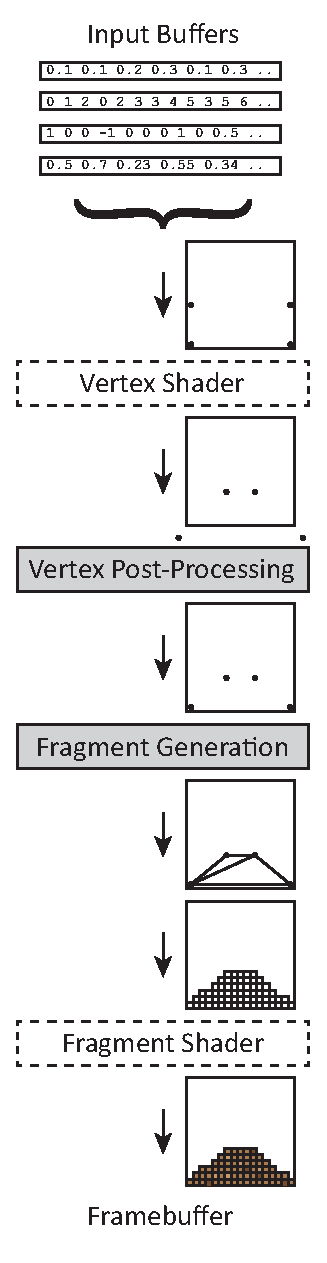
\includegraphics[scale=1.1]{images/pipeline-overview.eps}
}

The Vertex Shader runs once for every single vertex that is drawn. It is responsible for transforming (translating, scaling, rotating, etc.) individual vertices around the scene. This is for instance used to move objects around the scene, or to place them in desired locations. 

Additionally, the Vertex Shader is responsible for projecting the scene on to the camera. Projections are used to define how the world looks through the \emph{lens} of the camera. For example, a ``perspective projection'' causes objects that are further away from the camera to shrink in size, mimicking the way the human eye perceives a scene. Here is the effect of a perspective projection on a scene with two spheres:

\begin{figure}[htbp]
  \centering
  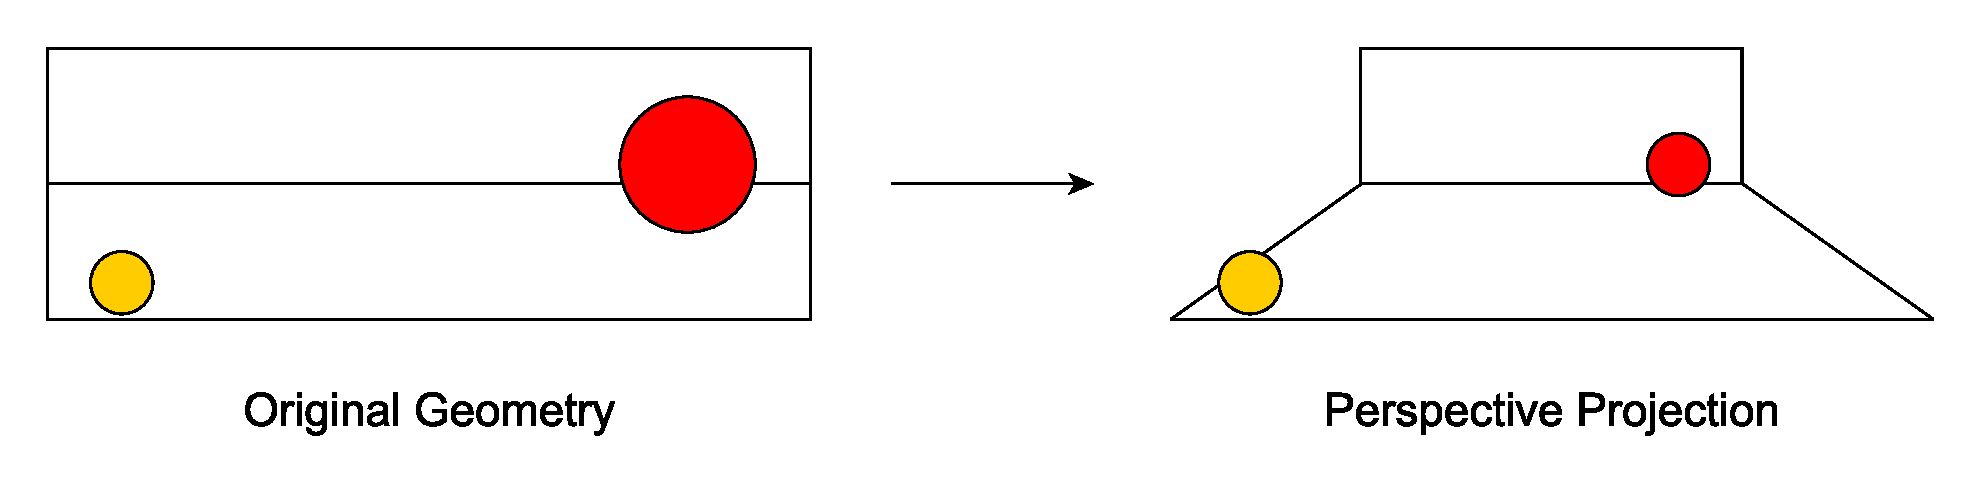
\includegraphics[scale=0.45]{images/openGL_perspective_projection.eps}
\end{figure}

After the Vertex Shader has finished processing all vertices, OpenGL uses the geometry specification to figure out which geometric primitives it should draw. These can either be points, lines or triangles. It then rasterises these primitives into pixels.

This is where the Fragment Shader comes in, which is responsible for determining the colour of each fragment. Fragments are pixels OpenGL attempts to draw. These may end up behind other geometry, thus not being visible in the final frame. They are thus not exactly the same thing as pixels on screen \footnote{The Direct3D equivalent of the Fragment Shader is called the ``Pixel Shader''. I suppose Microsoft ultimately calls it what it is, while OpenGL makes a distinction.}.

The Fragment Shader is executed once for {\bf every single} fragment. For complicated scenes this may imply rendering significantly more fragments than there are pixels on the screen.

\section{The GLSL Language}

So how exactly does one write a Shader? The OpenGL standard describes a language, imaginatively called the ``OpenGL Shading Language'', or GLSL for short.

GLSL is designed as a dialect of C, with a number of additions and limitations. We will therefore mainly look at the differences between these two languages. However, due to the extensive number of features in GLSL not all language components will be mentioned here for the sake of simplicity. As such you should not consider this overview complete or exhaustive, but it should include everything you need to complete the assignments.

\newpage

\subsection{General Layout of a Shader}

A minimal Shader source file commonly follows a specific layout. This layout has been outlined below:

\begin{minted}{glsl}
#version xxx
// Line 1: GLSL version declaration (this *HAS* to be line 1!)

// Input/output variable declaration
// For example: 
in layout(location=2) vec3 vertex;

// A main function
void main() {
	// Do things
}
\end{minted}

As you can see, there's a version declaration of which version of GLSL you are using, as well as a listing of what input values are required and returned by the Shader. Finally, the main function represents the entry point of the Shader. Note that unlike some versions of C, the main function in GLSL always returns \mintinline{glsl}{void}.

We'll take a look at each of these parts in the sections below.

\subsection{The \#version Statement}

The first line in every Shader {\bf must} be a declaration of which version of GLSL the Shader is written in. There have been a number of iterations of GLSL over the years, some of which have significantly changed the language syntax. 

We are using OpenGL 4.0 or higher in these labs, so the version statement should reflect that. For example, putting \mintinline{glsl}{#version 400} at the top of a shader file will cause OpenGL to use the revision of GLSL that accompanies OpenGL 4.0. If your graphics card can support it, I'd recommend using \mintinline{glsl}{#version 450} by default.

\subsection{The Input/Output Declaration}

Because the Vertex and Fragment Shaders are programmable stages of the OpenGL pipeline, they require input for their operation and are expected to produce certain kinds of output depending on their place in the pipeline. 

OpenGL requires these inputs and outputs to be defined as global variables in the Shader. To mark a variable as an input or output, you have to use the \mintinline{glsl}{in} and \mintinline{glsl}{out} keywords respectively, as shown below:

\begin{minted}{glsl}
in vec4 vertex;
out vec4 transformedVertex;
\end{minted}

Because OpenGL tries to be both helpful and versatile, the Vertex and Fragment Shader both require you to define different inputs and outputs. However, you can add inputs and outputs at will for your own purposes. Here's an overview of what you have to define in each case:

\begin{description}
  \item[Vertex Shader input:] \hfill \\
  You need to explicitly define input variables for any Vertex Attributes you specified in the VAO you'd like to render. Note that if you want to pass any additional attributes to the Fragment Shader, you also have to define those as inputs here, and assign them to the output variables in the Shader code. This will cause them to be passed on to the Fragment Shader.
  \item[Vertex Shader output:] \hfill \\ 
  You are required to somewhere in your Shader code set the predefined output variable \mintinline{glsl}{out vec4 gl_Position} containing the transformed location of the vertex being processed by the Shader. In addition, you can define additional outputs that will be passed on to the Fragment Shader in case additional values are required for calculating the colours of pixels.
  \item[Fragment Shader input:] \hfill \\
  Any values that have been explicitly passed on from the Vertex Shader. Note that because the Vertex Shader is only executed for every vertex instead of every pixel, values from different vertices are interpolated automatically by OpenGL before they are passed into the Fragment Shader.

  This can be turned off if desired (see the OpenGL documentation for details), but is in the vast majority of cases a useful feature.
  \item[Fragment Shader output:] \hfill \\ 
  Usually only a single \mintinline{glsl}{vec4} with RGBA format containing the colour of the fragment (pixel). Note that in GLSL all colour channel values range between 0 and 1. 
\end{description}

As mentioned previously, the VAO we specified contains vertex attribute with specific indices. The Vertex Shader must indicate which input variable should originate from which Vertex Attribute. 

OpenGL therefore contains a ``layout'' mechanism to identify these correspondences. If you look at the \mintinline{c}{glVertexAttribPointer()} function specification, the first parameter requires you to specify an index. To ensure that the correct Vertex Attribute is connected to the correct shader input, you just have to ensure that the index specified in \mintinline{c}{glVertexAttribPointer()} matches with the index of the shader input variable.

The easiest way for accomplishing this is to use the \mintinline{glsl}{layout(location=[index])} qualifier before your input declaration. For example, if we would like the input variable to correspond to a buffer with index 6, we can define the input variable as follows:

\begin{minted}{glsl}
in layout(location=6) vec4 vertex;
\end{minted}

If you want to pass on values to another Shader further down the pipeline, such as the Fragment Shader, you will also need to specify layout qualifiers, in the same way as you did for connecting vertex attributes to Shader inputs. You have to make sure that the output index of the Vertex Shader matches the input index of the Fragment Shader to ensure OpenGL understands this output and input correspond to each other. 

For illustration, the following output variable in the Vertex Shader:

\begin{minted}{glsl}
layout(location=2) out vec4 colour;
\end{minted}

Would correspond to this input variable in the Fragment Shader:

\begin{minted}{glsl}
layout(location=2) in vec4 thisNameCanBeDifferent;
\end{minted}

For reference, here's an overview over the entire pipeline:

\vspace{0.5cm}
\centerline {
  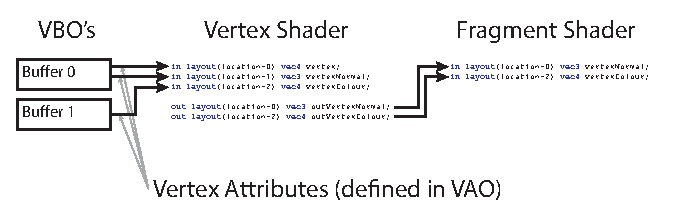
\includegraphics[scale=1.4]{images/overview.eps}
}
\vspace{0.5cm}

Note, however, that the layout qualifier feature is only available from OpenGL 4.3 or higher. If your graphics card and driver does not support this version, or you have configured Gloom to use an earlier version (it currently uses version 4.0 by default), you need to use a different method.

In this case there are two options.

First, it is possible to let OpenGL automatically determine the indices at which Vertex Attributes should be assigned. You can accomplish this by leaving out the location specification in the Shader source.

Next, ensure that your Shader is loaded and bound before you construct your VAO(s). You can now use the \mintinline{c}{glGetAttribLocation()} function to obtain the indexes which OpenGL has assigned to your inputs:

\begin{minted}{c}
int glGetAttribLocation(unsigned int programID, char* variableName);
\end{minted}

The first parameter is the ID of your Shader Program (these are explained in more detail in section \ref{sec:loadshader}), and the second is a string containing the name of the Shader's input variable. You should set the indexes passed in to \mintinline{c}{glVertexAttribPointer()} and \mintinline{c}{glEnableVertexAttribArray()} while setting up the VAO.

Alternatively, after compiling the shaders, but before linking them, it is possible to specify the input locations by calling the function \mintinline{c}{glBindAttribLocation()}. This function replaces the effect of layout specification syntax.

Of the two alternatives, this method is superior. However, it requires modification to the shader loading function supplied in Gloom. You can decide yourself which solution works best for you. All three methods are considered correct in the context of the grading of these labs.

\subsubsection{Uniforms}

There is another ``special'' kind of input to a Shader; the uniform variable. You can consider uniforms to be \emph{parameters} that are the same for every instance of your Shader that's being executed. Hence the name ``uniform''. 

You can use them to pass in a value of any type supported by GLSL into a Shader. They act as constants while the Shader is executing. You can thus only read from them from within the Shader itself. One application of uniforms is to define values that are the same throughout a single draw call, but still change from time to time. 

The value of a Uniform is kept between executions of the shader. It retains its value until it is changed. Note that this must always be done on the CPU side. Shader code is unable to change uniform values. Also note that GLSL considers uniforms inputs to your Shader. You should therefore specify positions for them explicitly, like you did with the inputs and outputs before. Here's an example: 

\begin{minted}{glsl}
uniform layout(location = 3) vec4 lightPosition;
\end{minted}

You can subsequently use the glUniform[number of elements][parameter datatype]() function to set the value(s) of the uniform. For the uniform defined above, this is how you can set its value in OpenGL:

\begin{minted}{c}
// Function used: 
// void glUniform4f(int index, 
//             float value1, float value2, float value3, float value4);
// Note that we above defined the location of the uniform to be 3
glUniform4f(3, 1f, 2f, 3f, 4f);
\end{minted}

If the layout specification syntax is not supported on your machine, you can use the \mintinline{c}{glGetUniformLocation()} function to obtain the index assigned to the input by OpenGL. An overview over the most relevant \mintinline{c}{glUniform()} function signatures is shown in table \ref{tab:uniforms}.

\begin{sidewaystable}
  \centering
\caption{A table showing the function signatures of the most commonly used flavours of glUniform().}
\label{tab:uniforms}
\begin{tabular}{|l|l|l|l|}
\hline
\textbf{Input Data Type} & \textbf{C Data Type} & \textbf{GLSL Data Type} & \textbf{Function Signature} \\ \hline
float & \begin{tabular}[c]{@{}l@{}}float\\ glm::vec2\\ glm::vec3\\ glm::vec4\end{tabular} & \begin{tabular}[c]{@{}l@{}}float\\ vec2\\ vec3\\ vec4\end{tabular} & \begin{tabular}[c]{@{}l@{}}void glUniform1f(int location, float v0);\\ void glUniform2f(int location, float v0, float v1);\\ void glUniform3f(int location, float v0, float v1, float v2);\\ void glUniform4f(int location, float v0, float v1, float v2, float v3);\end{tabular} \\ \hline
int & \begin{tabular}[c]{@{}l@{}}int\\ glm::int2\\ glm::int3\\ glm::int4\end{tabular} & \begin{tabular}[c]{@{}l@{}}int\\ int2\\ int3\\ int4\end{tabular} & \begin{tabular}[c]{@{}l@{}}void glUniform1i(int location, int v0);\\ void glUniform2i(int location, int v0, int v1);\\ void glUniform3i(int location, int v0, int v1, int v2);\\ void glUniform4i(int location, int v0, int v1, int v2, int v3);\end{tabular} \\ \hline
float matrix & \begin{tabular}[c]{@{}l@{}}glm::mat2x2\\ glm::mat3x3\\ glm::mat4x4\end{tabular} & \begin{tabular}[c]{@{}l@{}}mat2\\ mat3\\ mat4\end{tabular} & \begin{tabular}[c]{@{}l@{}}void glUniformMatrix2fv(int location, int count, bool transpose, float* value);\\ void glUniformMatrix3fv(int location, int count, bool transpose, float* value);\\ void glUniformMatrix4fv(int location, int count, bool transpose, float* value);\end{tabular} \\ \hline
\end{tabular}
\end{sidewaystable}

\subsection{Data Types}

There exist five basic datatypes in GLSL: \mintinline{glsl}{bool}, \mintinline{glsl}{int}, \mintinline{glsl}{uint}, \mintinline{glsl}{float} and \mintinline{glsl}{double}. Note that unlike C, integers are specified to be 32-bit values. Also, most modern graphics cards do not natively support double precision values, or are extremely slow at processing them (for a modern high-end card this can be a factor of 32 slower compared to single precision values). You'll therefore want to default to single precision whenever you need to work with floating point values, unless your \emph{really} need the precision.

GLSL also includes vector and matrix types for conveniently grouping data together. 

The most commonly used vector types are \mintinline{glsl}{vec2}, \mintinline{glsl}{vec3} and \mintinline{glsl}{vec4}, containing 2, 3 and 4 single precision floats respectively. You can create a new vector like this:
\begin{minted}{glsl}
vec4 vector = vec4(1.0, 0.0, 0.0, 1.0);
\end{minted}
And access individual elements like this:
\begin{minted}{glsl}
// method 1: use the built-in rgba components
float element0 = vector.r;
float element1 = vector.g;
float element2 = vector.b;
float element3 = vector.a;

// method 2: use the built-in xyzw components:
float element0 = vector.x;
float element1 = vector.y;
float element2 = vector.z;
float element3 = vector.w;

// method 3: use array indices:
float element0 = vector[0];
float element1 = vector[1];
float element2 = vector[2];
float element3 = vector[3];
\end{minted}

If you only need certain elements of the vector, you can also combine different properties like this:

\begin{minted}{glsl}
vec2 location2D = vector.xy;
vec3 colour = vector.rgb;
\end{minted}

Besides vectors, GLSL also contains built-in matrix types. These types are formatted as ``mat[number of columns]x[number of rows]''. For instance, the type of a matrix with 3 rows and 2 columns would be \mintinline{glsl}{mat2x3}. Unlike vector types, there is only one method for accessing matrices. 

Also note that matrices in OpenGL are column major. If you're not familiar with the term, column major means that you first address the column, then the row when dealing with multidimensional arrays, such as matrices. 

Here's a snippet of code showing how to use them:

\begin{minted}{glsl}
// defines the matrix: [1, 2]
//                     [3, 4]
mat2x2 matrix = {{1, 3}, {2, 4}};
// changes it to: [1, 2]
//                [5, 4]
matrix[0][1] = 5.0;
\end{minted}

%Finally, if you would like to use textures in your Shader, you have to pass their ID into the Shader as a uniform variable. The type of this uniform will not be an integer, but a \mintinline{glsl}{sampler2D}. If you want to sample a pixel in your texture, you have to use the \mintinline{glsl}{texture()} function. Here's how to use it:

%\begin{minted}{glsl}
%in layout(location = 4) sampler2D sampler;

%void main() {
%    // Texture coordinates are usually defined by the geometry specification.
%    // So in practice you usually get these from the Vertex Shader.
%    vec2 textureCoordinates = vec2(0.5, 0.5);
%    vec4 texturePixelColour = texture(sampler, textureCoordinates);
%}
%\end{minted}

\subsection{Operators}

Even though most operators such as addition, subtraction or multiplication work exactly the same as in C, there are some notable differences with GLSL.

First of all, you can't typecast in GLSL in the way you can in C. Instead, you can in most cases call the type you want to convert to as a ``function''. Here's an example showing how to convert from a float to an int:

\begin{minted}{glsl}
int intValue = int(floatValue);
\end{minted}

Secondly, you can use the basic arithmetic operators (+, -, *, /) on matrices and vectors, or a combination of the two. Do note that this follows the rules of matrix multiplication. So addition performs element wise addition, given that the matrices or vectors are of equal dimensions.

Here's some examples:
\begin{minted}{glsl}
// Creates a 4x4 matrix with 1's in the leading diagonal; 
// the identity matrix.
mat4x4 matrix = mat4(1); 

vec3 positionXYZ = vec3(1, 2, 3);
vec4 positionXYZW = vec4(1, 2, 3, 1);

// Compilation error: a 4x4 matrix can't be multiplied with a 3x1 matrix
vec4 error = matrix * positionXYZ; 

// returns vec4(1, 2, 3, 1) as anything multiplied with the 
// identity matrix results in the same matrix.
vec4 newPosition = matrix * positionXYZW; 

// returns vec3(2, 4, 6)
vec3 doublePosition = 2 * positionXYZ; 
\end{minted}


\subsection{Language Constructs}

The remainder of GLSL should pretty much be downhill from here on out, because it's practically the same as C :)

But let's go over them for the sake of reference.

First of all, the if statement. You really want to avoid these as much as possible, as the branch instructions generated by if statements are incredibly expensive on GPUs. Especially considering that the Vertex and Fragment Shaders are executed many times per frame.

Moreover, modern GPUs tend to cluster cores together in order to allow them to share part of the processor logic. This for instance includes instruction decoding. It allows the size of each individual core to be shrunk, and as a result more cores can fit on the die.

This also affects the way shaders are executed. Specifically, if a branch instruction causes some cores to choose the \emph{if} clause and some the \emph{else} clause, \emph{both} clauses are executed. Cores which chose the \emph{else} clause will need to wait until the \emph{if} clause is finished, and vice versa. As such you don't get a speedup in the execution of your shader the way you would if it were executed on a CPU. It may even cause a slowdown.

\begin{minted}{glsl}
if(someVariable > 3) {
	// Do something
} else {
	// Do something else.
}
\end{minted}

The same is true for for loops. If you need the performance, it's usually better to look for alternate strategies or redundancies to avoid having to use branching.

\begin{minted}{glsl}
for(int i = 0; i < 10; i++) {
	// Do something
}
\end{minted}

That also counts for the while loop:

\begin{minted}{glsl}
while(someCondition != false) {
	// Do something
}
\end{minted}

And finally, you can define additional functions if you need them:

\begin{minted}{glsl}
bool isGreaterThan(float a, float b) {
	return a > b;
}
\end{minted}

\section{Loading and using Shaders}
\label{sec:loadshader}

You've hopefully gotten a sense at this point on how to write a Shader. Now we should take a look at how to set them up and use them. 

In terms of the lab work, doing this yourself is not required, though if you want to implement the procedure yourself you're welcome to do so. An implementation of the shader loading procedure has been implemented for you in the file Shader.hpp.

As opposed to Direct3D's shader model, OpenGL has opted for a local compilation approach. This means that whenever you want to use a shader on the user's machine, you have to compile it locally. Major graphics card vendors therefore include GLSL compilers in their graphics drivers.

This may sound like an odd decision at first. After all, why do you not compile it once on your development machine, and save everyone else the effort? 

The problem is that modern graphics hardware differs from vendor to vendor. The binary code generated by each vendor's compiler may differ significantly. Local compilation avoids tricky situations where you have to compile explicitly for each vendor's card, possibly even different models. Local compilation is therefore a more fitting approach. 

\subsection{The Shader Program Object}

In OpenGL shaders are grouped together into so-called \emph{Program Objects}. The idea is that each shader is compiled individually, attached to a Program Object and finally linked together. Once set up, Program Objects can be activated at will.

The linking stage is responsible for checking that shader combinations are compatible. That is, that one shader's output specifications match with another shader's input specification.

The resulting structure looks something like this:

\centerline {
  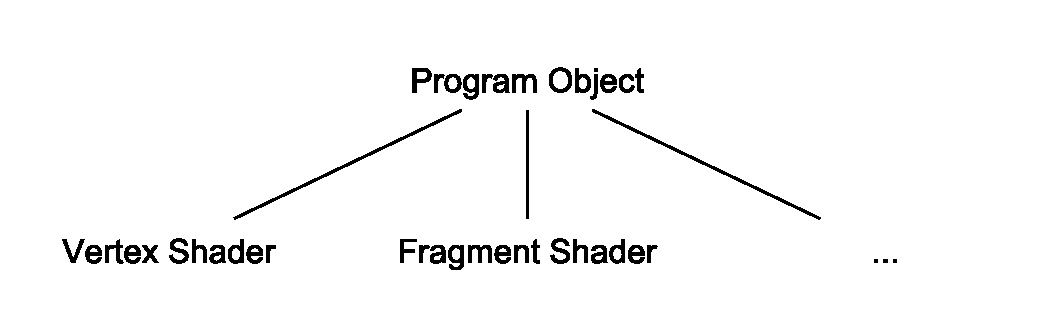
\includegraphics[scale=0.6]{images/openGL_program_structure.eps}
}

First off, we create a new Program Object using:

\begin{minted}{c}
unsigned int glCreateProgram();
\end{minted}

Once again, the function does not return a structure or object, but an ID that can be used to refer to the object in OpenGL calls.

\subsection{Loading and Compiling a Shader}

Next, we need to load and compile each of the shaders we would like to use. OpenGL does not provide any means for loading shader source code from a file, so loading a text file into memory is your responsibility. 

Hint: it may be useful to drop the loading of a single shader in its own function as the process is nearly identical for each shader type.

Compiling a shader starts with the creation of a Shader object:

\begin{minted}{c}
unsigned int glCreateShader(enum shaderType);
\end{minted}

The shaderType parameter specifies the type of shader you are creating. Some relevant options are:

\begin{itemize}
  \item \mintinline{c}{GL_VERTEX_SHADER}
  \item \mintinline{c}{GL_FRAGMENT_SHADER}
\end{itemize}

Next we pass in the source code of the shader Program using:

\begin{minted}{c}
void glShaderSource(
        unsigned int shaderID, 
        int count, 
        char** strings, 
        int** lengths
);
\end{minted}

The \mintinline{c}{shaderID} parameter is the ID returned by \mintinline{c}{glCreateShader()}.

The source string itself can either be one large string, or chopped up into smaller bits. Appending them all together should give the complete source code of the Shader.

\mintinline{c}{Count} represents the number of parts you have divided the Shader source code into. \mintinline{c}{Strings} and \mintinline{c}{lengths} are arrays of strings and integers, respectively. \mintinline{c}{Strings} contains the actual source code, and \mintinline{c}{lengths} the length of each string in \mintinline{c}{strings}. 

Now that the source code is in place, we can compile it using:

\begin{minted}{c}
void glCompileShader(unsigned int shaderID);
\end{minted}

Although you're strictly not required to, it's very good practice to check for compilation errors. 

You can check whether compiler errors occurred using:

\begin{minted}{c}
int shaderCompilationStatus = 0;

// glGetShaderiv() allows requesting information about a shader.
// In this case the compilation status (GL_TRUE if success, GL_FALSE if not)
glGetShaderiv(shaderID, GL_COMPILE_STATUS, &shaderCompilationStatus);

bool compilationErrorsOccurred = shaderCompilationStatus == GL_FALSE;
\end{minted}

If an error occurred, you can obtain an information log using:

\begin{minted}{c}
int logLength = 0;

// Again using glGetShaderiv() for obtaining the log length
glGetShaderiv(shaderID, GL_INFO_LOG_LENGTH, &logLength);

// Allocating enough memory to store the info log
char* infoLog = (char*) malloc(logLength);

glGetShaderInfoLog(shaderID, logLength, NULL, infoLog);

// Print the info log:
printf("A Shader compilation error occurred. Info log:\n");
printf("%s\n", infoLog);

free(infoLog);
\end{minted}

You can delete a shader to free up memory if the shader is not going to be used for a significant stretch of time. You can do so using:

\begin{minted}{c}
void glDeleteShader(unsigned int shaderID);
\end{minted}

And we're done! Run this process for both the Vertex and Fragment shaders, and we can move on to the linking stage of compilation.

\subsection{Attaching and Linking Shaders}

After compiling both shaders, you have to attach each shader to the Program object you created. The \mintinline{c}{glAttachShader()} function does just that:

\begin{minted}{c}
void glAttachShader(unsigned int programID, unsigned int shaderID);
\end{minted}

This will make Shaders a part of the Program Object. 

Now that all shaders have been attached to the Program Object, we can perform the linking stage of compilation:

\begin{minted}{c}
void glLinkProgram(unsigned int programID);
\end{minted}

Again, it is strictly not necessary to check for linking errors, but doing so is considered good practice. The process is almost identical compared to Shader compilation error checking. You can obtain the linking status of your Program by calling:

\begin{minted}{c}
int programLinkStatus = 0;

glGetProgramiv(programID, GL_LINK_STATUS, &programLinkStatus);
bool linkingFailed = programLinkStatus == GL_FALSE;
\end{minted}

Obtaining the error log is also the same compared to Shaders, apart from the OpenGL function calls:

\begin{minted}{c}
int logLength = 0;

// Using glGetProgramiv() instead of glGetSDhaderiv().
// The functions have the same intent; obtaining information
// about the Program and Shader, respectively.
glGetProgramiv(programID, GL_INFO_LOG_LENGTH, &logLength);

// Allocating enough memory to store the info log
char* infoLog = (char*) malloc(logLength);

glGetProgramInfoLog(shaderID, logLength, NULL, infoLog);

// Print the info log:
printf("Program linking failed. Info log:\n");
printf("%s\n", infoLog);

free(infoLog);
\end{minted}

And that's it. We can now use the Program object at will. When enabled, the Shaders you defined will take their respective places in the OpenGL pipeline, and do whatever you have instructed them to do.

\subsection{Enabling and Disabling the Program Object}

The only thing that now remains is the question of how to activate your Program Object. This can be done by calling:

\begin{minted}{c}
void glUseProgram(unsigned int programID);
\end{minted}

Passing in your programID will activate it. Passing in 0 will restore OpenGL's default behaviour.

\subsection{Debugging Shaders}

Because shaders are executed in such large quantities and communication between the CPU and GPU is complicated, it is very difficult to debug one. The Fragment Shader is in my own experience the most complicated one to get right, so I tend to use the fragment colour as a debug value. 

For instance, if a value becomes inexplicably large, you can insert an if statement that checks for such large values. It can then set the pixel colour to red, which makes it visible to you.

Another tip is to read your shader's source code. Shader code tends to (and should!) be very short. The problem space is therefore usually much smaller than typical CPU code. Careful reading can therefore get you quite far.

Some graphics card vendors supply debug tools for their card which you can also give a try.